%!TEX root = 0.main.tex

\section{The Belkin's trinity}
\subsection{Towards a theoretical foundation of Laplacian-based manifold methods}

In this paper they present two results: a pointwise probabilistic convergence of \textbf{the extension of the graph Laplacian} 
\begin{definition}{Graph Laplacian}
	$$ \left(\mathbf L_n^t\right)_{ij}=\begin{cases}
	-w_{ij}, & i\neq j\\
	\sum_{k}w_{ik}, & i=j
	\end{cases}$$
\end{definition}
\begin{definition}{Point cloud Laplace operator}
	$$L_n^t:\quad(L_n^tf)(y) = \frac{1}{n}f(y)\sum_i e^\frac{||x_i-y||}{4t}-\frac{1}{n}\sum_ie^\frac{||x_i-y||}{4t}f(x_i)$$
\end{definition}
\begin{definition}{Functional approximation to the Laplace-Beltrami operator} \label{eq:L^t}
	$$L^tf(p) :=  \frac{1}{ (4\pi t)^{\frac{k+2}{2}}} \int_\mathcal Me^{-\frac{||p-x||^2}{4t}}\left(f(x)-f(p)\right)d\mu(x)$$
\end{definition}

\begin{theorem}{Pointwise convergence}
	$$\forall f \in C^\infty(\mathcal M)\quad  C\frac{(4\pi t_n)^{-\frac{k+2}{2}}}{n} L_n^t f(\bf x) \xrightarrow{n\to\infty}\triangle_\mathcal M f(\bf x)$$
\end{theorem}


and a uniform (pointwise convergence of the operator) one
\begin{theorem}{uniform convergence}
	$$\sup_{x\in\mathcal M, f\in \mathcal F_C}\left| C\frac{(4\pi t_n)^{-\frac{k+2}{2}}}{n} L_n^t f(\bf x) - \triangle_\mathcal M f(\bf x) \right|\xrightarrow{n\to\infty}0
	, \quad \mathcal F_C = \left\{f\in C^\infty(\mathcal M), f^{(i)}(x)\leq M, i=1,2,3\right\}$$
\end{theorem}


here nothing is said about convergence of the spectra, plus there's nothing written about the relationship between $\mathbf{Eig} L_n^t$ (the eigenfunctions and eigenvalues of the extension of the graph Laplacian) and $\mathbf {Eig} \mathbf {L}_n^t$ (the eigenvectors and eigenvalues of the matrix Laplacian).

Theorem 1 is proven by simple analysis arguments and by Hoeffding's formula (probability). 
First, by the simple law of large numbers, we have that for a fixed $t>0$, a fixed function $f$ and a fixed point $p\in\mathcal M$
\begin{equation}\label{eq:pointwise convergence of laplacian discrete approximation}
\lim_{n\to\infty}\frac{1}{tn}\frac{1}{ (4\pi t)^{\frac{k}{2}}}L_n^tf(p)= L^tf(p)
\end{equation}




To prove the convergence of $L^t$ to $\triangle_\mathcal M$, then we need three steps, that we can recycle completely. They use the fact that thanks to the exponential map the heat kernel centered on $p$ on any manifold can be approximated by a Gaussian in the ambient Euclidean space in a small neighborhood of $p$, and the relationship between Euclidean distances and geodesic distances.

\textbf{In order to adapt this proof to our needs, we just need to find an alternative to the law of large numbers (LLN) used to prove \ref{eq:pointwise convergence of laplacian discrete approximation}}

Theorem 2 is proven with arguments of Functional Analysis: Ascoli-Arzelà, compact convergence in Sobolev spaces, etc.etc...

\subsection{Consistency of Spectral Clustering}
 $$ \mathbf{Eig} \mathbf{L}^t_n \xrightarrow[a.s.]{n\to\infty} \mathbf{Eig} L^t $$
It aims at proving the convergence of eigenvalues and eigenvectors of random graph Laplacian matrices for growing sample size. They present two results: one for the normalized Laplacian and one for the unnormalized Laplacian. Since the matrix eigenvectors grow in dimension as the sample size increases, standard convergence arguments can not be applied. However, they show that there exists a function $f\in C(\mathcal M)$ such that the difference between the eigenvector $v_n$ and the restriction of $f$ to the sample converges to $0$

$$||v_n-\rho_nf||\rightarrow 0$$

To do so they see the eigenvector $v_n$ as the restriction to the sample of a continuous eigenfunction $f_n$ of some continuous operator $U'_n$ that acts on the space $C(\mathcal M)$. Then they use the fact that 

$$||v_n-\rho_nf||_\infty = ||\rho_nf_n-\rho_nf||_\infty\leq ||f_n-f||_\infty$$


So, it will just be necessary to show that  $$||f_n-f||_\infty\rightarrow 0$$
 \textbf{compact convergence} of both matrices towards $L^t$ (where $\mathcal M$ is a compact metric space) in the Banach space of the continuous functions $(C, ||\cdot||_\infty)$. 

Compact convergence ensures convergence of spectral properties in the following sense: for isolated eigenvalues of the limit operator $\triangle_\mathcal M$ with finite multiplicity we have convergence of eigenvalues and eigenspaces but not convergence of eigenfunctions. for isolated simple eigenvalues of the limit operator we have also convergence of the eigenfunctions!

The proof consists in three steps:
\paragraph{Step 1} Construct a bounded operator $U'_n$ on the Banach space $(C(\mathcal M), ||\cdot||_\infty)$ such that restricted on the sampled values behaves like $\mathbf{L}'_n$. Then, construct an operator $U'$ such that for the law of large numbers for a fixed $f$ and for a fixed $x$, $U'_nf(x) \xrightarrow U'f(x) $
\paragraph{Step 2} Here they establishes the connection between the spectra of $L'_n$ and $U'_n$. In particular, they prove a one-to-one correspondence between the eigenfunctions and eigenvalues of $U'_n$ and the eigenvectors and eigenvalues of $L'_n$, provided that satisfy $\lambda\notin \{1\}=\sigma_{ess}(U'_n)= \sigma_{ess}(U')$.
\paragraph{Step 3} Here we prove compact convergence:

$$U'_n \xrightarrow[n\to\infty]{c,\ a.s.}U'$$

At the light of compact convergence and on the analysis of the essential spectrum of $U'_n, U'$ and the one-to-one correspondence of the spectra done in step 2, given Proposition 6 \textit{Perturbation results for compact convergence} we get to the following result

\begin{theorem}
	Let $\lambda\neq 1 $ be an eigenvalue of $U'$ and $M\subset \mathbb C$ an open neighborhood of $\lambda$ such that $\sigma(U')\cap M=\{\lambda\}$. Then:
\begin{enumerate}
	\item Convergence of eigenvalues: The eigenvalues in$\sigma(L'_n)\cap M$ converge to $\lambda$ in the sense that every sequence $(\lambda_n)_{n\in\mathbb N}$ with $\lambda_n\in\sigma(L'_n)\cap M$ satisfies $\lambda_n\rightarrow \lambda$ almost surely.
	\item Convergence of spectral projections: There exists some $N\in\mathbb N$ such that for $n>N$, the sets $\sigma(U'_n)\cap M$ are isolated in $\sigma(U'_n)$. For $n>N$, let $Pr'_n$ be the spectral projection of $U'_n$ corresponding to $\sigma(U'_n)\cap M$, and $Pr$ the spectral projection of $U$ for $\lambda$. Then $Pr'_n\xrightarrow p Pr a.s.$
	\item Convergence of eigenvectors: if $\lambda$ is a single eigenvalue, then the eigenvectors of $L'_n$ converge a.s. up to a change of sign: if $v_n$ is the eigenvector
	of $L'_n$ with eigenvalue $\lambda_n$, $v_{n,i}$ its i-th coordinate, and $f$ the eigenfunction of eigenvalue $\lambda$, then there exists a sequence $(a_n)_{n\in\mathbb N}$ with $a_i \in \{+1,-1\}$ such that $\sup_{i=1,...,n} |a_nv_{n,i} - f(X_i)| \rightarrow 0$ a.s. In particular, for all $b \in\mathbb R$, the sets $\{a_nf_n > b\}$ and $\{f > b\}$ converge, that is, their symmetric difference satisfies $P(\{f > b\}\triangle\{a_nf_n > b\}) \rightarrow 0$.
\end{enumerate}
\end{theorem}

A similar theorem is stated also for non-normalized Laplacian matrix, although the arguments stay the same.
\subsection{Convergence of Laplacian Eigenmaps}
Here all the pieces are put together. 

 $$ \mathbf{Eig} \mathbf{ L}^t_n \xrightarrow[a.s.]{n\to\infty} \mathbf{Eig} L^t \xrightarrow{t\to0} \mathbf{Eig} \triangle_\mathcal M $$
 
 \begin{theorem}
 	Let $\lambda_{n,i}^t$ be the ith eigenvalue of $\hat L_n^t$ and $e^t_{n,i}$ be the corresponding eigenfunction (which for each fixed i will be shown to exist for t sufficiently small). Let $\lambda_{i}$ be the ith eigenvalue of $\triangle_\mathcal M$ and $e_{i}$ be the corresponding eigenfunction. Then there exists a sequence $t_n\rightarrow 0$ such that
 	
 	$$\lim_{n\rightarrow\infty} \lambda_{n,i}^{t_n}=\lambda_i$$
 	$$\lim_{n\rightarrow\infty}||e_{n,i}^{t_n}(x) - e_i(x)||_2 = 0$$
 	
 	where the limits are in probability.
 	
 \end{theorem}

\paragraph{Step 1: Spectral convergence of the empirical approximation $\mathbf{ L}_n^t$ to $L^t$}
Recycle the work of \textbf{Consistency of Spectral Clustering} with the analysis of the essential spectrum of the limit operator $\sigma_{ess}(L^t)$.
\paragraph{Step 2: Spectral convergence of the functional approximation $L^t$ to $\triangle$}
Really hard. Uniform operator convergence does not hold, however spectral convergence is still assured in theorem 4.1 of the paper. This part, although really hard, will stay the same!


\section{Pointwise convergence in the HEALPix case}

Getting inspired from the work flow presented above, we try to replicate the first theorem obtained in \textbf{Towards a theoretical foundation of Laplacian-based manifold methods} but not in the case of random Laplacians, but in the case of deterministic ones where the sampling is given by the HEALPix scheme. This analysis will be a preparatory work to further studies, since as we pointed out so far, from this kind of convergence nothing is said about the convergence of eigenvalues and eigenvectors. However, this study could maybe tell us something about the equivariance of the graph with respect to the action of the rotation group $SO(3)$.


We remind that \textbf{in order to adapt this proof to our needs, we need to find an another inequality to substitute Hoeffding's inequality.}


\paragraph{Definitions}

$n$ defines the number of vertices in the graph, $N$ defines the parameter $N_{side}$
\begin{definition}{Graph Laplacian}
	$$ \left(\mathbf L_n^t\right)_{ij}=\begin{cases}
	-w_{ij}, & i\neq j\\
	\sum_{k}w_{ik}, & i=j
	\end{cases}$$
\end{definition}
\begin{definition}{Point cloud Laplace operator}
	$$L_n^t:\quad(L_n^tf)(y) = \frac{1}{n}\left[ \sum_{i=0}^{n-1} e^\frac{||x_i-y||}{4t}\left(f(y)-f(x_i)\right)\right]$$
\end{definition}
\begin{definition}{Functional approximation to the Laplace-Beltrami operator} \label{eq: my L^t}
	$$L^t:\quad L^tf(y) := \int_{\mathcal S_2}e^{-\frac{||p-x||^2}{4t}}\left(f(y)-f(x)\right)d\mu(x)$$
\end{definition}

\paragraph{Step 1: keeping $t$ fixed.}

Here we want to prove that 
$$\forall f \text{ Lipschiz,}\quad \forall y\in\mathcal S_2,  \quad\quad L_n^tf(y)\rightarrow \frac{1}{|\mathcal S_2|}\int e^{-\frac{||x-y||^2}{4t}}\left(f(y)-f(x)\right)d\mu(x) = \frac{1}{|\mathcal S_2|} L^tf(y)$$

This will be an easy but introductory result to the main result proved in Step 2.

\begin{proof}
We know by construction that the HEALPix sampling cut the sphere into equal areas. Let us note the surface of one level $S_N$, and the maximum distance to the center point of one surface\textbf{ $d_{N}$}.
Let us assume that the function $f$ is $L$ Lipschitz, we have
\[
\int_{\sigma_{i}}f({\bf x})\text{d}{\bf x}-\frac{1}{2}Ld_{N}S_{N}\leq S_{N}f({\bf x}_{i})\leq\int_{\sigma_{i}}f({\bf x})\text{d}{\bf x}+\frac{1}{2}Ld_{N}S_{N}.
\]
Hence we have:
\[
\sum_{i}\int_{\sigma_{i}}f({\bf x})\text{d}{\bf x}-\sum_{i}\frac{1}{2}Ld_{N}S_{N}\leq S_{N}\sum_{i}f({\bf x}_{i})\leq\sum_{i}\int_{\sigma_{i}}f({\bf x})\text{d}{\bf x}+\sum_{i}\frac{1}{2}Ld_{N}S_{N}
\]
and 
\[
\left|S_{N}\sum_{i}f({\bf x}_{i})-\int f({\bf x})\text{d}{\bf x}\right|\le\frac{1}{2}Ld_{N}S_{tot}
\]
where $S_{tot}$ is the the total surface of the sphere. Now we need to characterize $d_{N}$ with respect of $N$ and $L$ with respect of $m$ and $\ell$. 


\begin{tcolorbox}
	Now, we found the following code, part of Healpix\_cxx 2.15a \cite{Healpix_cc} that illustrates how to calculate the maximum distance between a pixel and the corner of the corresponding patch. The class \lstinline|vec3| implements a 3D cartesian vector, the function \lstinline|vec3.set_z_phi(double, double)| creates a unit vector from a z coordinate and an azimuthal angle. Both \lstinline|va| and \lstinline|vb| converge towards the point $(2/3, 0)$, making $$d_{N}\rightarrow0$$
	\begin{lstlisting}[language=c++]
	double Healpix_Base::max_pixrad() const
	{
	vec3 va,vb;
	va.set_z_phi (2./3., pi/(4*nside_));
	double t1 = 1.-1./nside_;
	t1*=t1;
	vb.set_z_phi (1-t1/3, 0);
	return v_angle(va,vb);
	}
	\end{lstlisting}
	$\mathcal S_{N} = \{x_i\}  \text{ set of points of the HEALPix sampling scheme for a fixed }N$,\\$c_i = \text{farthest corner of the area patch associated to the pixel }x_i$, we have that 
	$$\hat d=\max_{x_i\in \mathcal S_{N}}d(x_i, c_i) \leq ||v_a-v_b||\rightarrow 0$$
	where $v_a = (2/3, \pi/N)$, $v_b = (1-t_1/3, 0)$ and $t_1=(1-1/N)^2$.
\end{tcolorbox} 

Thanks to this result, we have the following two point wise convergences

$$\forall f \text{ Lipschiz,}\quad \forall y\in\mathcal S_2,  \quad\quad \frac{1}{n}\sum_i e^{-\frac{||x_i-y||^2}{4t}}\rightarrow \frac{1}{|\mathcal S_2|}\int e^{-\frac{||x-y||^2}{4t}}d\mu(x)$$
$$\forall f \text{ Lipschiz,}\quad \forall y\in\mathcal S_2,  \quad\quad \frac{1}{n}\sum_i e^{-\frac{||x_i-y||^2}{4t}}f(x_i)\rightarrow \frac{1}{|\mathcal S_2|}\int e^{-\frac{||x-y||^2}{4t}}f(x)d\mu(x)$$

Remembering the definition of the extension of the graph Laplacian we have the following point wise convergence:
$$\forall f \text{ Lipschiz,}\quad \forall y\in\mathcal S_2,  \quad\quad L_n^tf(y)\rightarrow \frac{1}{|\mathcal S_2|}\int e^{-\frac{||x-y||^2}{4t}}\left(f(y)-f(x)\right)d\mu(x) = \frac{1}{|\mathcal S_2|} L^tf(y)$$
\end{proof}
\paragraph{Step 2: replacing Hoeffding's inequality}
\begin{figure}[h!]
	\label{fig:Belkin proof}
	\caption{Old proof we need to modify}
	\centering
	\fbox{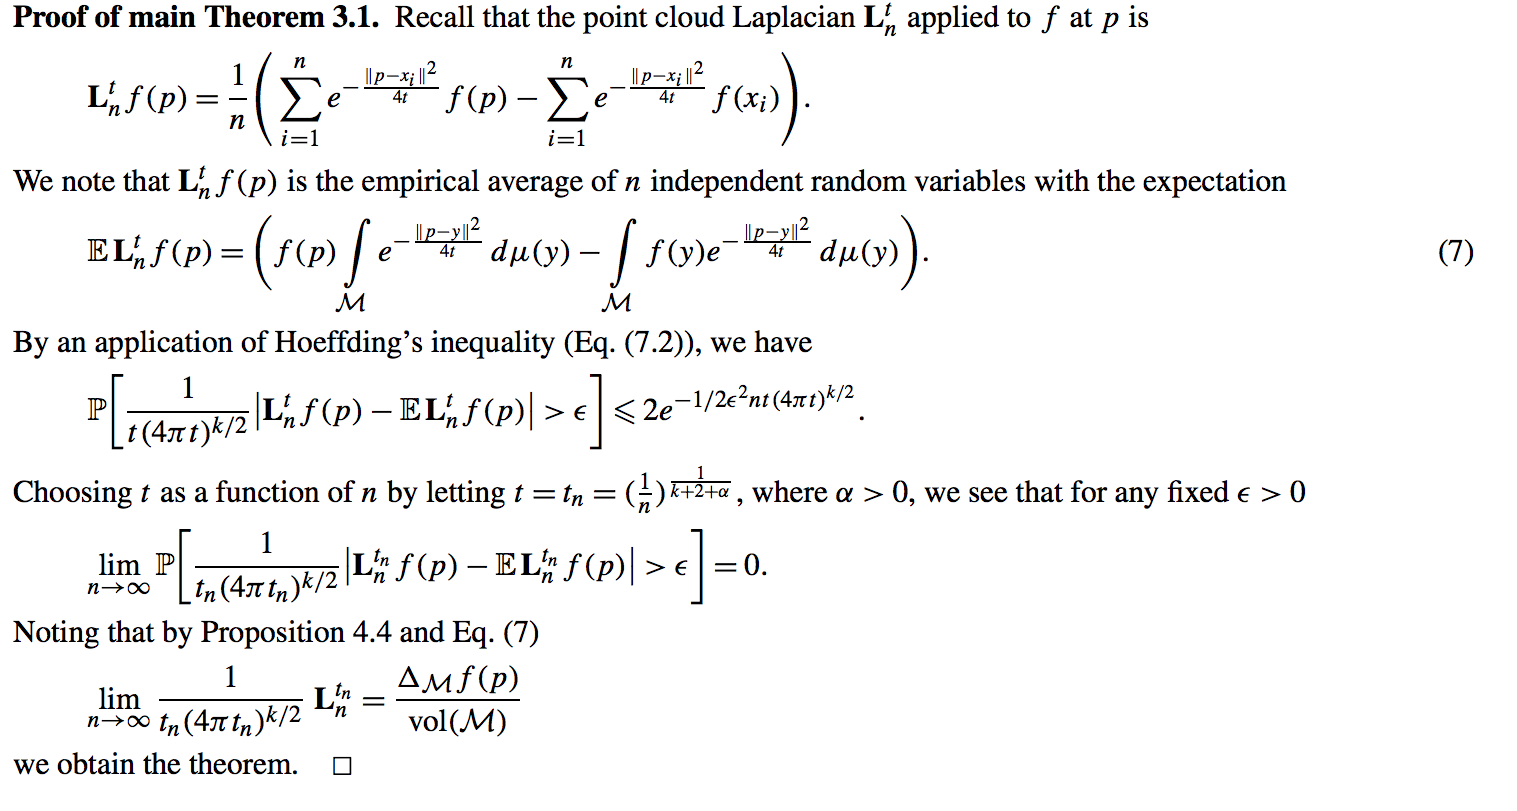
\includegraphics[width=0.9\textwidth]{Figs/03/oldproof.png}}
\end{figure}
In the previous paragraph we already proved that \textit{keeping t fixed} $L_n^tf(x)\rightarrow L^tf(x)$. We now want to prove the following thing:
$$\left|\frac{1}{4\pi t^2}\left(L_n^tf(x) - \frac{1}{|\mathcal S_2|}L^tf(x)\right)\right|\xrightarrow[n\to \infty]{t\to 0}0$$
\textit{for $t\to0$ and $n\to\infty$ at the same time}. In other words, we want to prove that there exists a sequence $(t_n), \lim_{n\to\infty}t_n=0$ such that 
$$\forall f \text{ Lipschitz, } \forall x\in\mathcal S_2 \quad \left|\frac{1}{4\pi t_n^2}\left(L_n^{t_n}f(x) -\frac{1}{|\mathcal S_2|} L^{t_n}f(x)\right)\right|\xrightarrow{n\to \infty}0$$

\begin{proof}
	
	We define for simplicity of notation
	$$\phi^t(x;y) := e^{-\frac{||x-y||^2}{4t}}\left(f(y)-f(x)\right)$$
	$$K^t(x,y) :=  e^{-\frac{||x-y||^2}{4t}}$$
	$$N := N_{side}$$
	
	we start by writing the following chain of inequalities
	$$||L_n^tf-\frac{1}{|\mathcal S_2|}L^tf||_\infty = \max _{y\in \mathcal S_2} \left|L_n^tf-\frac{1}{|\mathcal S_2|}L^tf\right|=$$
	$$= \max _{y\in \mathcal S_2} \left| \frac{1}{n} \sum_{i=1}^n \phi^t(x_i; y)-\frac{1}{|\mathcal S_2|} \int_{\mathcal S_2} \phi^t(x;y)d\mu(x) \right|$$
	$$\leq \max _{y\in \mathcal S_2} \sum_{i=1}^n  \left| \frac{1}{n}  \phi^t(x_i; y)-\frac{1}{|\mathcal S_2|} \int_{A_i} \phi^t(x;y)d\mu(x) \right|$$
	$$= \frac{1}{|\mathcal S_2|} \max _{y\in \mathcal S_2} \sum_{i=1}^n  \left| \frac{|\mathcal S_2|}{n}  \phi^t(x_i; y)-\int_{A_i} \phi^t(x;y)d\mu(x) \right|$$
	$$= \frac{1}{|\mathcal S_2|} \max _{y\in \mathcal S_2} \sum_{i=1}^n  \left| A_i  \phi^t(x_i; y)-\int_{A_i} \phi^t(x;y)d\mu(x) \right|$$
	$$\leq \frac{1}{|\mathcal S_2|} \max _{y\in \mathcal S_2} \left[ n \mathcal L_{\phi^t_y} \max_{i=1,...n} (d_i|A_i|)  \right]$$
	
	where $\mathcal L_{\phi^t_y}$ is the Lipschitz constant of $x \rightarrow \phi^t(x, y)$ and where we used for the last inequality the arguments used in Step 1. If we assume $\max_{i=1,...n} (d_i|A_i|) \leq \frac{C}{N^3}$ (meaning $\max_{i=1,...n} d_i \leq \frac{C}{\sqrt{n}}$ and $\max_{i=1,...n} |A_i| \leq \frac{C}{n}$)
	and remember that for HEALPix $n=12N^2$
	
	$$\leq \frac{1}{|\mathcal S_2|} \max _{y\in \mathcal S_2} \left[ 12 \mathcal L_{\phi^t_y} \frac{C}{N} \right]$$
	
	Let's now find the explicit dependence $t\rightarrow \mathcal L_{\phi^t_y}$
	
	$\mathcal L_{\phi^t_y} = ||\partial_x\phi^t(x;y)||_\infty = ||\partial_x\left(K^t(x;y)f(x)\right)||_\infty = ||\partial_x K^t(x;y)f(x) + K^t(x;y)\partial_x f(x)||_\infty \leq$
	
	$ \leq ||\partial_x K^t(x;y)f(x)||_\infty + ||K^t(x;y)\partial_x f(x)||_\infty \leq  ||\partial_x K^t(x;y)||_\infty||f(x)||_\infty + ||K^t(x;y)||_\infty||\partial_x f(x)||_\infty = $
	
	$ = ||\partial_x K^t(x;y)||_\infty||f(x)||_\infty + ||\partial_x f(x)||_\infty = \mathcal L_{K^t_y} ||f||_\infty + ||\partial_xf||_\infty = \mathcal L_{K^t_y} ||f||_\infty + \mathcal L_f$
	
	where $\mathcal L_{K^t_y}$ is the Lipschitz constant of $x\rightarrow K^t(x;y)$. We can observe that such constant does not depend on $y$. Thus
	
	$\mathcal L_{K^t_y} = \norm{\partial_x e^{-\frac{x^2}{4t}}}_\infty = \norm{\frac{x}{2t}e^{-\frac{x^2}{4t}}}_\infty = \left. \frac{x}{2t}e^{-\frac{x^2}{4t}}\right|_{x=\sqrt{2t}}=(2et)^{-\frac{1}{2}}\propto t ^ {-\frac{1}{2}}$
	
	So we can continue
	
	$$ \frac{1}{|\mathcal S_2|} \max _{y\in \mathcal S_2} \left[ 12 \mathcal L_{\phi^t_y} \frac{C}{N} \right]\leq$$
	$$ \leq \frac{1}{|\mathcal S_2|} \left[   \frac{12C}{N} \left( (2et)^{-\frac{1}{2}} \norm{f}_\infty + \mathcal L_f \right)\right]\leq$$
	$$  \leq \frac{1}{|\mathcal S_2|} \frac{12C\norm{f}_\infty}{N(2et)^\frac{1}{2}} +   \frac{1}{|\mathcal S_2|} \frac{12C}{N}\mathcal L_f$$
	
	So we have that, rescaling by a factor $\frac{1}{t}\frac{1}{(4\pi t)^{\frac{k}{2}}}$
	
	$$\left.\norm{\frac{1}{t}\frac{1}{(4\pi t)^{\frac{k}{2}}}\left(L_n^tf-\frac{1}{|\mathcal S_2|}L^tf\right)}_\infty\right|_{k=2}\leq$$
	$$\leq \frac{1}{4\pi t^2}\norm{\left(L_n^tf-\frac{1}{|\mathcal S_2|}L^tf\right)}_\infty \leq$$
	$$ \leq \frac{3C}{\pi |\mathcal S_2|}\left[\frac{\norm{f}}{\sqrt{2e}}\frac{1}{Nt^\frac{5}{2}} + \frac{\mathcal L_f}{Nt^2}\right]$$
	
	we want $\begin{cases}
	t \rightarrow 0\\
	N \rightarrow \infty\\
	Nt^\frac{5}{2} \rightarrow \infty\\
	Nt^2 \rightarrow \infty
	\end{cases}$ in order for $ \frac{3C}{\pi |\mathcal S_2|}\left[\frac{\norm{f}}{\sqrt{2e}}\frac{1}{Nt^\frac{5}{2}} + \frac{\mathcal L_f}{Nt^2}\right] \xrightarrow[t\to 0 ]{N\to\infty}0$
	
	This is true if $\begin{cases}
	t(N) = N^\beta, &\beta\in(-\frac{2}{5}, 0) \\
	t(N) = N^\beta, &\beta\in(-\frac{1}{2}, 0)
	\end{cases} \implies t(N) = N^\beta, \quad \beta\in(-\frac{2}{5}, 0)$
	
	Indeed 
	
	$Nt^\frac{5}{2}=N^{\frac{5}{2}\beta+1}\xrightarrow{N \to \infty} \infty$ since $\frac{5}{2}\beta+1>0 \iff \beta>-\frac{2}{5}$
	
	$Nt^2=N^{2\beta+1}\xrightarrow {N \to \infty} \infty$ since $2\beta+1>0 \iff \beta>-\frac{1}{2}$
	
	So, for $t=N^\beta$ with $\beta\in(-\frac{2}{5}, 0)$ we have that 
	
	$$\begin{cases}
	(t_N)\xrightarrow{N\to\infty}0\\
	\norm{\frac{1}{4\pi t_N^2}L_n^{t_N}f-\frac{1}{|\mathcal S_2|}\frac{1}{4\pi t_N^2}L^{t_N}f}_\infty  \xrightarrow{N\to\infty}0
	\end{cases}$$

	
thanks to the fact that - proof in \cite{Belkin:2005:TTF:2138147.2138189} - 
	$$\frac{1}{4\pi t^2} L^tf(y) \xrightarrow{t\to 0 } \frac{1}{|\mathcal S_2|}\triangle_{\mathcal S_2}f(y)$$
	we conclude that
	$$\forall y\in\mathcal S_2 \quad \lim_{N\to\infty}\frac{1}{4\pi t_N^2} L_n^{t_N}f(y) =  \lim_{N\to\infty}\frac{1}{|\mathcal S_2|}\frac{1}{4\pi t_N^2} L^{t_N}f(y) = \frac{1}{|\mathcal S_2|^2}\triangle_{\mathcal S_2}f(y) $$
\end{proof}
